%\pagestyle{myheadings} %\markright{Linear Systems}
\chapter{Descriptive Statistics}
\label{sectionDescriptiveStatistics}
\index{Statistics!Descriptive statistics}
%\label{sec.intro}  \setcounter{equation}{0}
%\markboth{\ref{sec.intro}.
%\titleref{sec.intro}}{}

\section{Representing Data}

Data comes to us in the form of \textit{observations} (i.e. measurements) which we write symbolically as a lower case letter along with a subscript. For example, suppose we have taken a total of $n$ observations. We have observation 1, observation 2, observation 3, $\hdots$, observation $n-1$ and observation $n$. By letting $x$ represent an observation, all $n$ observations can be represented as:
$$x_1,~x_2,~ \hdots ,~ x_n$$ where $x_i$ is an individual observation, and the index $i=1, \ldots , n$. Here $n$ is referred to as the \textit{sample size}. We can also represent this data in condensed form as:
$$x_i~: \ \ i=1, \hdots , n$$
or in tabular form as:
\begin{center}
\def\arraystretch{1.5}
\begin{tabular}{|c|c|c|c|c|} \hline
\textbf{Observation} &$x_1$&$x_2$&$\cdots$&$x_n$
 \\ \hline
\textbf{Index} &1&2&$\cdots$&$n$ \\ \hline
\end{tabular}
\end{center}
\hfill

\begin{example}
The amount of time per week that a student spends studying for  STAT*2060 was recorded over 5 weeks. The measurements recorded are 4, 3, 6, 20, 2.
Represent this information in tabular form.


\hfill\\
{\emph{\textbf{\underline{Solution:}}}}\\

\begin{center}
\def\arraystretch{1.5}
\begin{tabular}{|c|c|c|c|c|c|}\hline
\textbf{Observation} & 4 & 3 & 6 & 20 & 2
 \\ \hline
\textbf{Index} & 1 & 2 & 3 & 4 & 5 \\ \hline
\end{tabular}
\end{center}
Here $n=5,~x_1=4,~x_2=3,~x_3=6,~x_4=20,$ and $x_5=2$.

\end{example}

\section{Numerical Measures of Location}

\subsection{Mean}
\index{Mean}


The \textit{mean} (or more precisely the arithmetic mean) of a data set is obtained by adding up all of the observations and dividing by the sample size (number of observations). The mean is the typical average that we are all familiar with. sWe use the symbol $\bar{x}$ to represent the sample mean.

\begin{definition}[Sample Mean]	\index{Mean!Sample mean}
Let $x_{1}, ~x_{2}, ~x_{3}, ~\ldots , ~x_{n}$ represent a sample of $n$ observations.
The sample mean is given by:
\begin{equation}
{\fontfamily{serif}\selectfont 
	\bar{x} = \frac{ \displaystyle\sum_{i = 1}^{n} x_{i} }{n} = \frac{ x_{1} + x_{2} + \dots + x _{n} }{n}
}
\end{equation}
\end{definition}

\noindent
The symbol $\sum$ is referred to as \textit{capital sigma} and symbolizes summation.

\subsection{Median}

\begin{definition}[Median]	\index{Median}
The middle value of ordered data.
\end{definition}

The manner that the median is calculated depends on whether we have an odd or even number of observations.

\begin{skeleton}
Consider $n$ observations $x_{1},x_{2},~\cdots~,x_{n}$.
\begin{itemize}
\item[]	If $n$ is odd,
	\begin{equation*}
	Median = \text{observation} \> \left( \frac{n + 1}{2} \right)
	\end{equation*} 
\item[]	If $n$ is even,
	\begin{equation*}
	Median = \text{average of observation} ~ \left(\frac{n}{2} \right) ~\text{and observation} ~ \left( \frac{n}{2} + 1 \right)
	\end{equation*} 
\end{itemize}
\end{skeleton}


\subsection{Mode}

\begin{definition}[Mode]	\index{Mode}
The most frequent observation(\textit{s}) relative to the rest of the data.
\end{definition}


\begin{nt}
The mean, median and mode are referred to as \textit{measures of central tendency} as they are indicators of how close the data is to the average and how spread out the data is.
\end{nt}




\subsection{Variance}	\index{Variance}

The variance is a measure of the squared distance relative to the mean.

\begin{definition}[Sample Variance]	
\index{Variance!Sample variance}
\index{Sample!Sample variance}
Let $x_{1},x_{2},x_{3}, ~\ldots~, x_{n}$ represent a sample of $n$ observations.
Let $\bar{x}$ represent the sample mean of this data.
The sample variance is given by:
	\begin{equation}
	\label{equationSampleVariance}
	s^{2} = \frac{ \displaystyle\sum_{i=1}^{n} (x_{i} - \bar{x})^{2} }{n - 1}  = \frac{ (x_{1} - \bar{x})^{2} +  (x_{2} - \bar{x})^{2} + \ldots + (x_{n} - \bar{x})^{2} }{n-1}
	\end{equation}
\end{definition}


\noindent
The variance is a non-negative value (i.e. the variance is always greater than or equal to zero).
Notice in equation $(\ref{equationSampleVariance})$ that we are taking a difference, then squaring the value obtained %\textit{before} 
before
summing all the terms together. 
If the term $x_{i} - \bar{x}$ were not squared, it would be possible to have both positive and negative values. That is, $x_{i}-\bar{x}$ would be positive if $x_{i} > \bar{x}$ and negative if $x_{i} < \bar{x}$. By squaring the $x_{i} - \bar{x}$ term, the formula will provide us with non-negative values.


\begin{nt}
An alternative (and sometimes easier) way to calculate variance is:

\begin{equation}\label{eqnSampleVariance}
	s^{2} =  \frac{ \displaystyle\sum_{i=1}^{n} x_{i}^2 -  \frac{ \bigg( \displaystyle\sum_{i=1}^{n} x_{i} \bigg)^{2} }{n} }{n - 1} % \quad \quad ~~ \circled{B}
\end{equation}
\end{nt}



\subsection{Standard Deviation}
\index{Standard deviation}

In the calculation of the sample variance given by equation ($\ref{eqnSampleVariance}$), the $x_i$ terms are squared. This means that the units of measurement are also squared. In order to get back to the original units of measurement we take the 
square root of the variance. This value is referred to as the \textit{standard deviation}.

\begin{definition}[Sample Standard Deviation]	
\index{Standard deviation!Sample standard deviation}
\index{Sample!Sample standard deviation}
Let $x_{1}, ~x_{2}, ~x_{3}, ~\ldots , ~x_{n}$ represent a sample of $n$ observations.
Let $s^{2}$ represent the sample variance of this data.
The sample standard deviation is given by:
	\begin{equation}
	s^{2} = + \sqrt{s^{2}}
	\end{equation}
\end{definition}

The standard deviation is a measure of the spread of the data relative to the mean. When we analyze data we typically describe the data in terms of the mean and standard deviation as the units are the same. However, the calculation of the sample variance is an important 
intermediate step.



\subsection{Percentiles}

\begin{definition}[Percentile]	\index{Percentile}
For ordered data, the $p^{th}$ percentile is the value such that p\% of all observations lie below it.
\end{definition}

Suppose that a student obtained a mark of 68\% on a test.
Although 68\% is not a very good grade, the test may have been difficult. Suppose you are told that this student who scored 68\% is in the $90^{th}$ percentile. This means that they scored better than 90\% of the rest of the class.

\subsection{Quartiles}


\begin{definition}[Quartile]	\index{Quartile}
In an ordered data set, quartiles are the three values that divide the data into four groups such that each group consists of one fourth of the data.
\end{definition}

The three quartiles are the first quartile ($Q_{1}$), second quartile ($Q_{2}$) and 
third quartile ($Q_{3}$) respectively.

\begin{itemize}
\item	First Quartile (Q$_{1}$)	:	A value such that 25\% (i.e. a quarter) of all observations lie below it.
\item	Second Quartile (Q$_{2}$)	:	A value such that 50\% (i.e. two quarters) of all observations lie below it.
\item	Third Quartile (Q$_{3}$)	:	A value such that 75\% (i.e. three quarters) of all observations lie below it.
\end{itemize}

The quartiles are actual specific percentiles. The first quartile is the $25^{th}$ percentile, the second quartile is the $50^{th}$ percentile and the third quartile is the $75^{th}$ percentile. Notice that the second quartile is the median. We do not have a fourth quartile. By using the definition of percentiles, the fourth quartile would be a value such that 100\% of all observations lie below it. This means that the fourth quartile is the largest value in the data set which is referred to as the \textit{maximum}.

\begin{definition}[Inter-Quartile Range]	\index{Inter-quartile range}
Let $Q_{1}$ and $Q_{3}$ represent the first and third quartiles of a data set respectively.
The inter-quartile range (IQR) is
	\begin{equation}
	IQR = Q_{3} - Q_{1}
	\end{equation}
\end{definition}

The inter-quartile range is a quick and simple measure of the dispersion of the data. The $IQR$ is also referred to as the \textit{mid-spread} since the difference between $Q_{3}$ and $Q_{1}$ contains 50\% of the data.The inter-quartile range is also used to calculate whiskers in boxplots which we will cover in section $\ref{sectionBoxplots}$.

\begin{nt}
The ``inter-quartile range'' should not be confused with the ``range''. The ``range'' of a data set is simply the difference between the largest value
and the smallest value.
\end{nt}


\begin{example}
Given a sample with the following $n=10$ observations,
\begin{center}
\begin{tabular}{cccccccccc}
9 & 4 & 1 & 10 & 8 & 11 & 15 & 6 & 6 & 16
\end{tabular} 
\end{center}
calculate the following.
\begin{benumerate}
\item The sample mean, $\bar{x}$. 
\begin{align*}
\bar{x} &= \sum_{i=1}^{n} \frac{x_i}{n} = \sum_{i=1}^{10} \frac{x_i}{10}\\
		&= \frac{9 + 4 + 1 + 10 + \hdots + 16}{10} = \frac{86}{10} = 8.6
\end{align*}
\item The sample median.
Rearranging the observations in ascending order,
\begin{center}
\begin{tabular}{cccccccccc}
1 & 4 & 6 & 6 & 8 & 9 & 10 & 11 & 15 & 16
\end{tabular} 
\end{center}
Since $n=10$ is even, the median is the average of ordered observation $\frac{n}{2} = \frac{10}{2} = 5$ and ordered observation $\frac{n}{2} + 1 = 6$. Therefore,
\[Median = \frac{8+9}{2} = \frac{17}{2} = 8.5\]
\item The sample variance, $s^2$, and sample standard deviation, $s$. 
\begin{align*}
s^2 &= \sum_{i=1}^{n} \frac{(x_i - \bar{x})^2}{n-1} = \sum_{i=1}^{10} \frac{(x_i-\bar{x})^2}{9} \\
	& = \frac{(9-8.6)^{2}+(4-8.6)^{2}+\hdots+(16-8.6)^{2}}{9} \\
	&= \frac{196.4}{9} = 21.82
\end{align*}
Alternatively,
\begin{align*}
&s^2 = \frac{\sum_{i=1}^{n} x_i^{2} - \frac{(\sum_{i=1}^{n} x_i)^2}{n}}{n-1} \\
&\sum_{i=1}^{n} x_i^{2} = 9^2 + 4^2 + 1^2 + \hdots + 16^2 = 936 \\
\end{align*}
From part(a),
\begin{align*}
&\sum_{i=1}^{n} x_i = 86 \\
&\Rightarrow s^2 = \frac{936-\frac{(86)^2}{10}}{9} = \frac{196.4}{9} = 21.82 \\
&\Rightarrow s = \sqrt{s^2} = \sqrt{21.82} = 4.67
\end{align*}

\item The first and third quartiles, $Q_1$ and $Q_3$. 

From part (b), the sample median is $8.5$. Splitting the ordered observations into two sets yields
\begin{center}
\def\arraystretch{1.5}
\begin{tabular}{ccccc}
1 & 4 & \underline{6} & 6 & 8 \\ 
9 & 10 & \underline{10} & 15 & 16
\end{tabular} 
\end{center}
Since both sets are of size $n=5$ which is odd, $Q_1$ and $Q_3$ are simply the medians of each set. That is, $Q_1 = 6$ and $Q_3 = 11$.
\item The inter-quartile range, IQR. 
\[ IQR = Q_3 - Q_1 = 11 - 6 = 5 \]
\end{benumerate}
\end{example}


\begin{example}
Sir Shoes-A-Lot is releasing a new running shoe in 3 months. The company wants to ensure that the shoe is competitively priced and collects the prices of nine similar shoes,
\begin{center}
\begin{tabular}{ccccccccc}
20.75 & 49.50 & 33.25 & 23.50 & 39.00 & 49.75 & 22.50 & 25.25 & 48.75
\end{tabular} 
\end{center}
\begin{benumerate}
\item What is the sample mean price?
\begin{align*}
\bar{x} &= \sum_{i=1}^{9} \frac{x_i}{9} \\
	&= \frac{20.75+49.50+33.25+\hdots+48.75}{9} \\
	&= \frac{312.20}{9} = 34.69
\end{align*}
\item What is the sample median price? 
Rearrange the prices in ascending order:
\begin{center}
\begin{tabular}{ccccccccc}
20.75 & 22.50 & 23.50 & 25.25 & 33.25 & 39.00 & 48.75 & 49.50 & 49.75
\end{tabular} 
\end{center}
Since $n=9$ is odd, the median price is equal to ordered observation number
\[ \frac{9+1}{2}=\frac{10}{2}=5\]
which is $33.25$.
\item What is the variance and standard deviation?
\begin{align*}
s^2 &= \sum_{i=1}^{9} \frac{\sum_{i=1}^{n} (x_i - \bar{x})^2}{n-1} \\
	&= \frac{(20.75-34.69)^2+(49.50-34.69)^2+\hdots+(48.75-34.69)^2}{8} \\
	&= \frac{1222.72}{8} = 152.72 \\
s &= \sqrt{s^2} = \sqrt{152.72} = 12.36
\end{align*}
\item What are $Q_1$ and $Q_3$?

From part (b), the median price is $33.25$. Splitting the data set into two sets yields
\begin{center}
\begin{tabular}{ccccc}
20.75 & 22.50 & \underline{23.50} & 25.25 & 33.25 \\ 
33.25 & 39.00 & \underline{48.75} & 49.50 & 49.75
\end{tabular} 
\end{center}
Since both sets are of size $n=5$ (odd), $Q_1=23.50$ and $Q_3 = 48.75$.
\item What is the inter-quartile range?
\[ IQR = 48.75 - 23.50 = 25.25 \]
\end{benumerate}
\end{example}



\section{Graphical Techniques}


Raw numbers on their own can be difficult to interpret.
Pictures and plots can be a very useful for representing information. Graphical representations of data provide us with a more intuitive method to
interpret information being analyzed.\\

Plots used for qualitative data include bar charts and pie charts.
Plots used for quantitative data include histograms, box plots and stem and leaf plots.
We can use plots to get a sense of the distribution our data follows as well
as visualize features such as spread, central tendency and unusual data points.

\begin{definition}[Skewness]	\index{Skewness}
Skewness is a measure of the symmetry of a distribution (i.e. how much a distribution leans towards a particular side).
\end{definition}

We can describe data as being left skewed, right skewed or symmetric. If the data is described as \textit{symmetric}, this implies that most observations are concentrated around the mean and tail off fairly evenly on both sides of the mean. If the data is described as \textit{right skewed} or \textit{positively skewed}, this implies that more observations are concentrated on smaller values and we observe a longer tail to the right side of the mean. If the data is described as \textit{left skewed} or \textit{negatively skewed}, this implies that more observations are concentrated on large values and we observe a longer tail to the left side of the mean.

\begin{nt}
Data that is right skewed may be referred to as being positively skewed and data that is left skewed may be referred to as being negatively skewed.
\end{nt}

\begin{figure}[H]
\begin{center}
	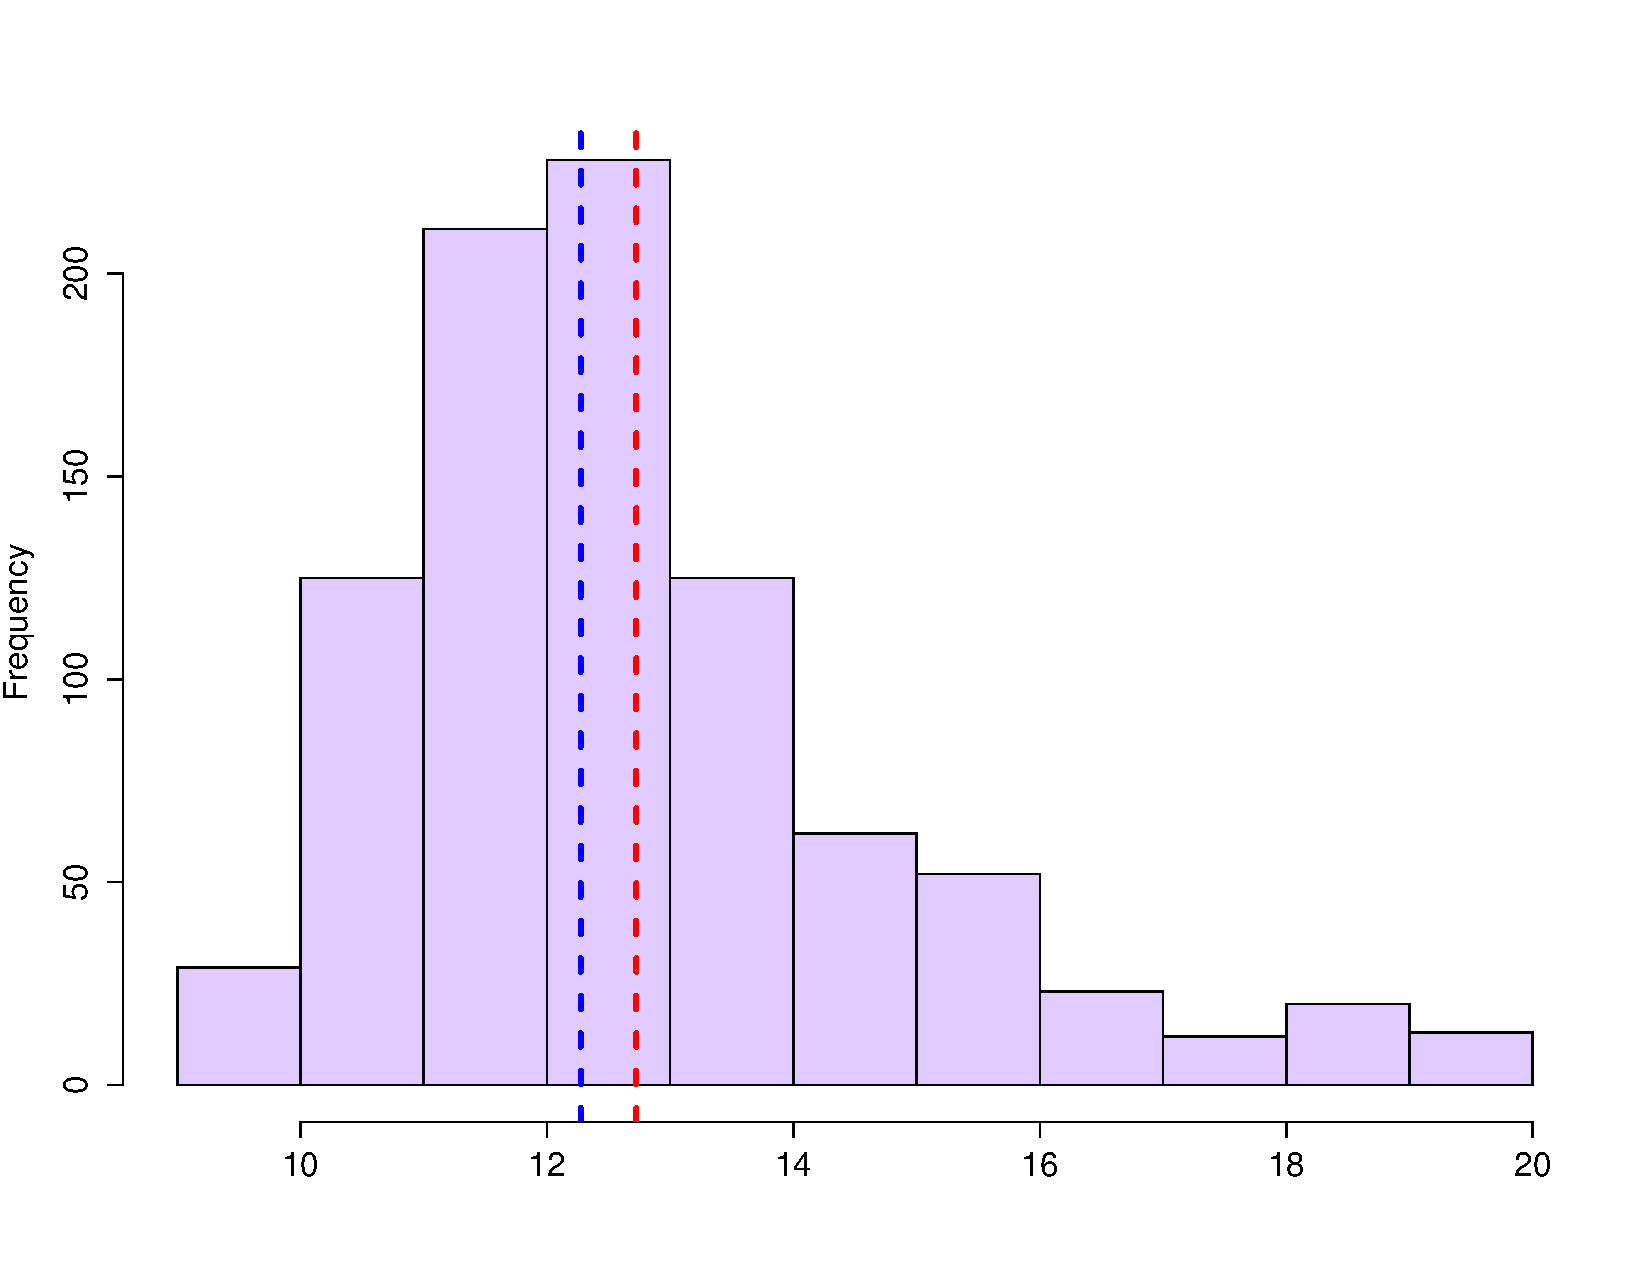
\includegraphics[scale=0.35]{Section2/skew_right.pdf}
\caption{When data is skewed right the mean (red) is larger than the median (blue) }
\end{center}
\end{figure}

\begin{figure}[H]
\begin{center}
	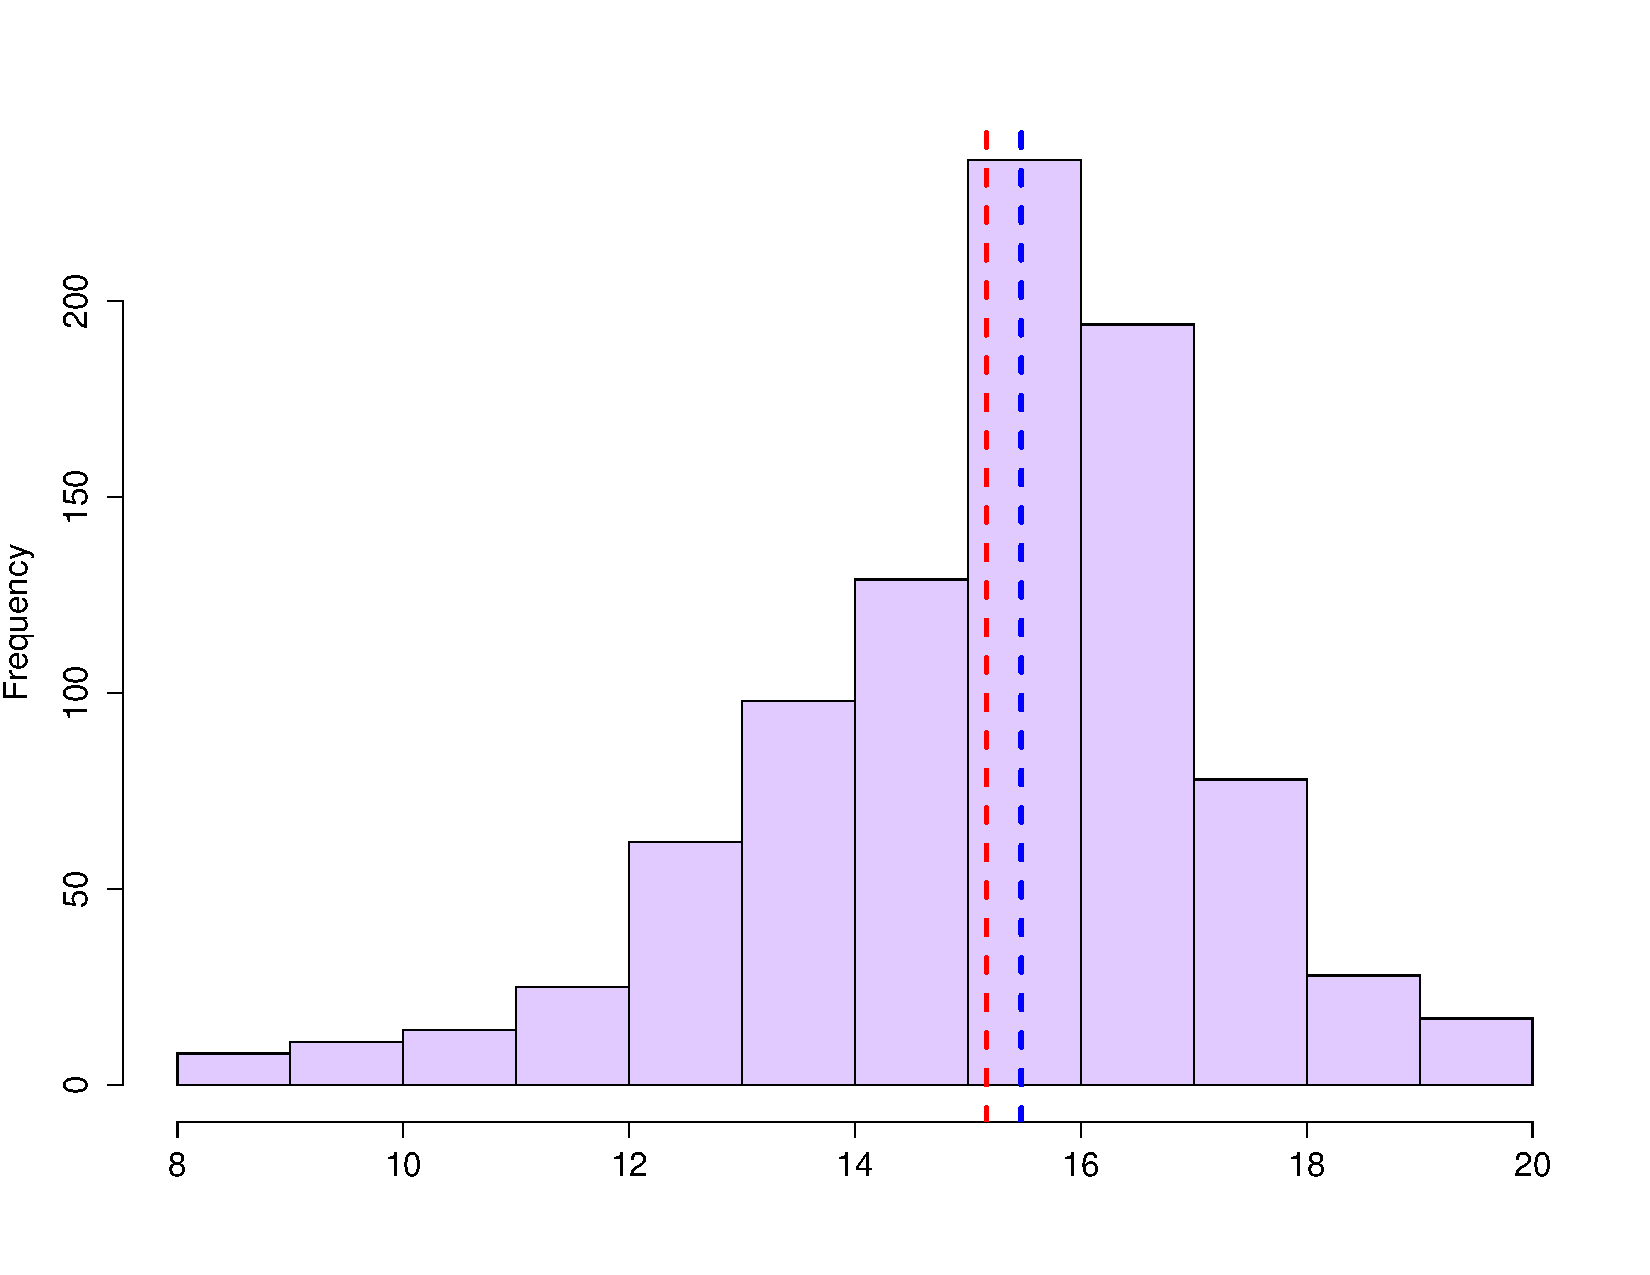
\includegraphics[scale=0.35]{Section2/skew_left.pdf}
\caption{When data is skewed left the mean (red) is smaller than the median (blue) }
\end{center}
\end{figure}

\begin{figure}[H]
\begin{center}
	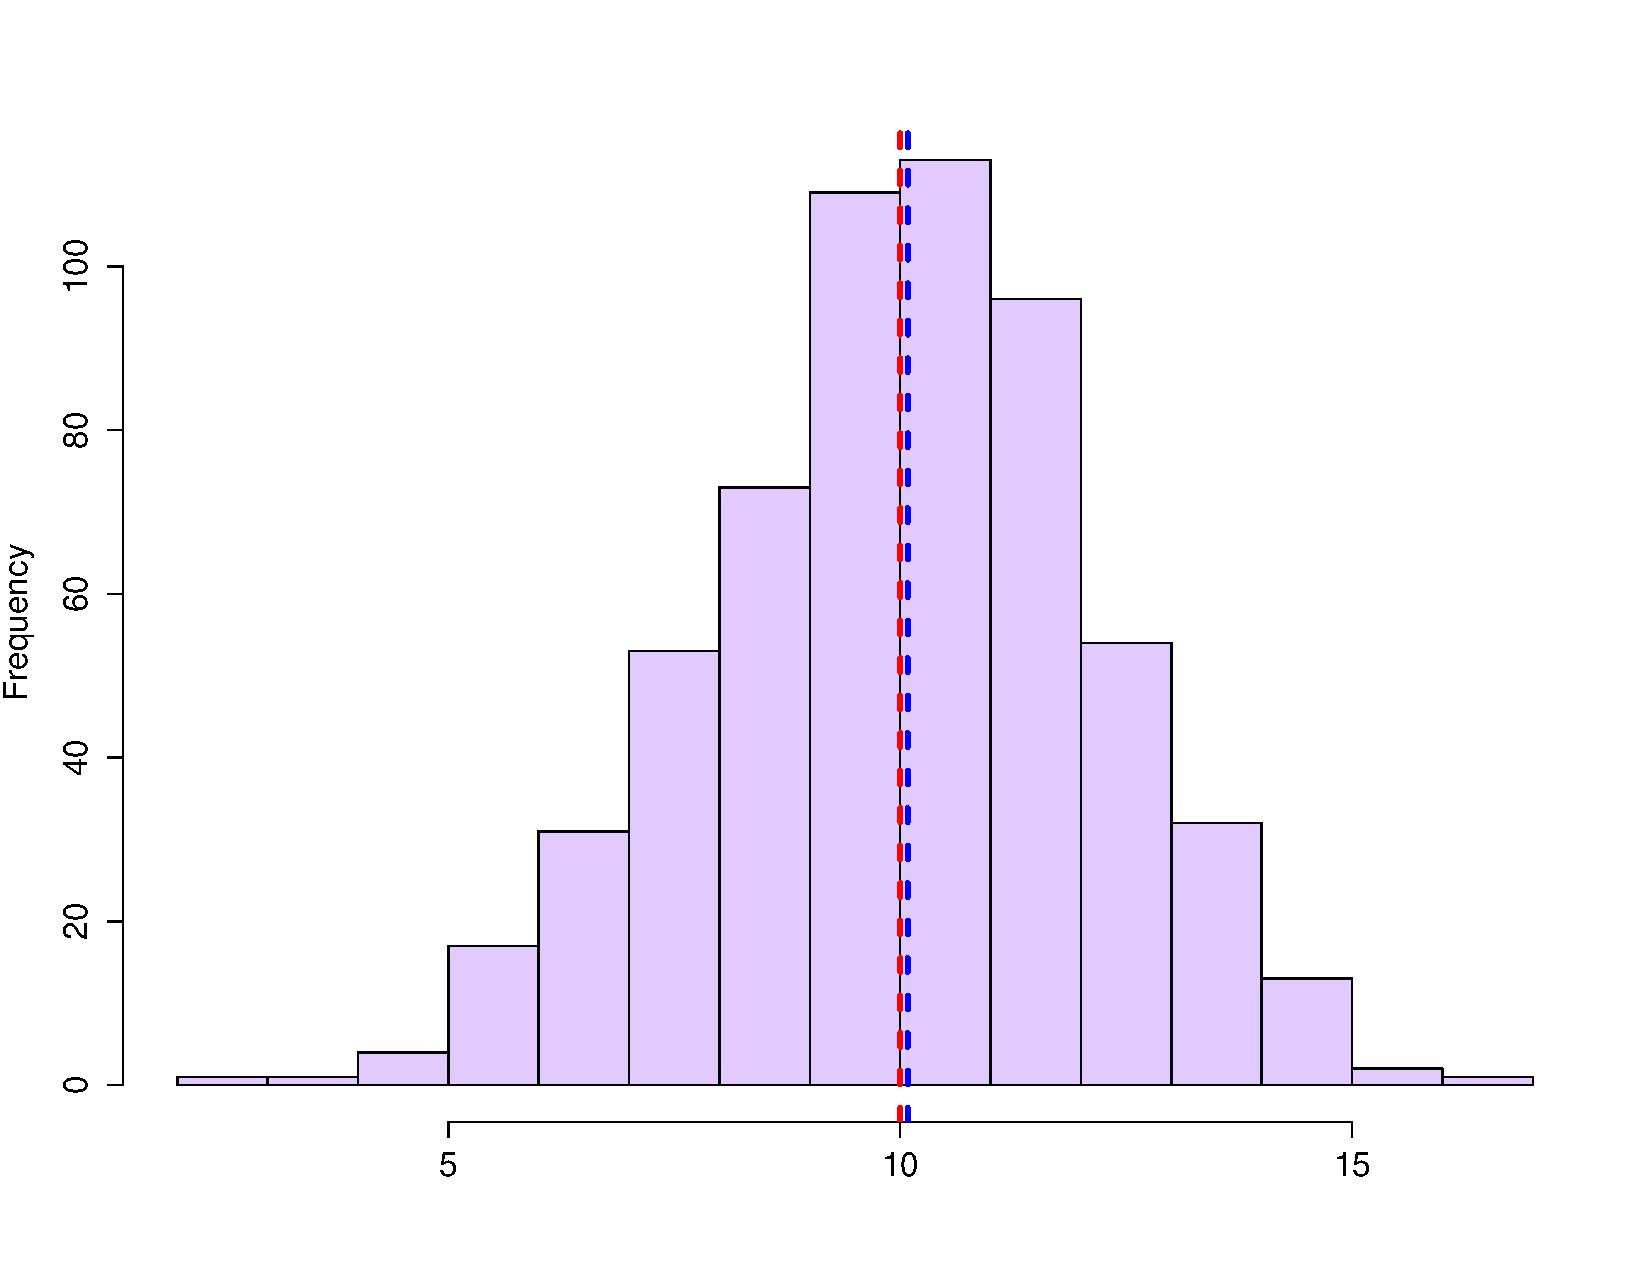
\includegraphics[scale=0.35]{Section2/symm.pdf}	
\caption{When data is symmetric the mean (red) is approximately equal the median (blue) }
\end{center}
\end{figure}

\begin{definition}[Outlier]	\index{Outlier}
An outlier is an unusual data point which appears to lies outside the overall pattern of the rest of the data.
\end{definition}

In other words, an outlier falls outside the range in which we would expect to see ``typical'' data values. Outliers may be present in data for a variety of reasons such as transcription error, measurement error, or we may have just measured a rare and unusual observation. In any case it is not a good practice to simply ignore outliers. All outliers should be investigated before deciding whether the observation should be included in data analysis or discarded.



\subsection{Histograms}	
\index{Histograms}
\index{Plots!Histograms}
Histograms and boxplots are useful tools which can (\textit{usually}) allow us to visually determine the skewness of a distribution. By noting skewness, we get even more information about our data. Note however that we may not always be able to determine skewness by visually observing a histogram. A histogram is similar to a bar chart with the distinction that histograms can only be created for \textit{quantitative} data.\\ 

The width of the bars does not have any numerical meaning for bar charts, 
however bar width matters for histograms.
They are an important factor in the creation of histograms. 
Interval width selection (or bin size selection) 
is an advanced topic that can be studied extensively and
there are several rules available to select interval widths.
However for the scope of this course we will keep things simple
and allow the reader to intuitively choose bin size.
After constructing a histogram, we can change the interval widths until
we feel that we have a picture that is a good representation of our data.\\

\noindent
In order to create a histogram, we must first
\begin{enumerate}
\item Construct class intervals (of equal or varying width) which will contain the data of interest.
\item Count the frequency at which data is observed in each of 
the class intervals.
\item Create a frequency table. A frequency tables contains both \textit{frequencies} and \textit{relative frequencies}. 
\end{enumerate}

\begin{definition}[Frequency]	\index{Frequency}
Frequency, $f_i$, is a count of the number of observations in each class interval $i$, $i=1,\hdots, m$.
\end{definition}

\begin{definition}[Relative Frequency]	\index{Frequency!Relative frequency}
Relative frequency, $r_i$, is the ratio of the frequency of class interval $i$, $f_i$, to the total frequency $F$ where
\[ F = \sum_{i=1}^{m} f_i \]
That is,
\[ r_i = \frac{f_i}{F} \; \; \; i= 1, \hdots, m \]
\end{definition}

Using our frequency table, we can create a \textit{frequency histogram} or a \textit{relative frequency histogram}. To create a frequency histogram, let the class intervals represent the width of the bars and the heights of these bars represent the frequencies of the data. To create a relative frequency histogram, let the class intervals represent the width of the bars and the heights of these bars represent the relative frequencies of the data.


\begin{nt}
When we use the term ``histogram'' on its own, we are usually referring to a frequency histogram.
\end{nt}


The general structure of a frequency table is given below.

\begin{center}
\def\arraystretch{1.15}
\begin{tabular}{c c c c l l}
Class			&	Freq.		&	Relative			&	&	Cumulative				&	Cumulative	\\
Interval			&			&	Freq.				&  	&	Freq.						&	Relative Freq.	\\
\hline
$[a_{1}, b_{1})$		&	$f_{1}$	&	$r_{1} = f_{1} / F$	& 	&	$f_{1}$					&	$r_{1}$\\
$[a_{2}, b_{2})$		&	$f_{2}$	&	$r_{2} = f_{2} / F$	&  	&	$f_{1} + f_{2}$				&	$r_{1}+r_{2}$\\
$[a_{3}, b_{3})$		&	$f_{3}$	&	$r_{3} = f_{3} / F$	& 	&	$f_{1} + f_{2} + f_{3}$		&	$r_{1}+r_{2}+r_{3}$\\
\vdots			&	\vdots	&	\vdots			&  	&	\hspace{0.75cm} \vdots		&	\hspace{0.75cm} \vdots\\
$[a_{m}, b_{m}]$	&	$f_{m}$	&	$r_{m} = f_{m} / F$	& 	&	$f_{1} + \ldots + f_{m} = F$	&	$r_{1} + \ldots + r_{m} = 1$\\
\hline
				&	$F = \displaystyle\sum_{i=1}^{m} f_{i}$ & 1 \\
\end{tabular}
\end{center}

\noindent
This may appear overwhelming however it is not as bad as it looks.
Lets do an example to illustrate.

\begin{example}
Suppose we have the following set of 30 observations which represents manufacturing times (in days) for mining equipment:
\begin{center}
\begin{tabular}{r r r r r r r r r r  }
53	& 	51	&	92	&	53	&	77	&	78	&	77	&	76	&	53	&	40	\\
45	&	60	&	99 	&	64 	&	44	&	93	&	64	&	45	&	53	&	26	\\
58	&	114	&	35	&	64	&	58	&	118	&	74	&	37	&	48	&	39	
\end{tabular}
\end{center}

It is hard to see any obvious patterns with just the raw data alone. Perhaps a picture will help. 
Construct a frequency histogram and a relative frequency histogram for this data. 

\hfill\\
{\emph{\textbf{\underline{Solution:}}}}\\

First we will begin by constructing a frequency table. An optional (but very useful) step is to sort the data.
\begin{center}
\begin{tabular}{r r r r r r r r r r  }
26	&	35	&	37	&	39	&	40	&	44	&	45	&	45	&	48	&	51	\\
53	&	53	&	53	&	53	&	58	&	58	&	60	&	64	&	64	&	64	\\
74  	&	76	&	77	&	77	&	78	&	92	&	93	&	99	&	114	&	118
\end{tabular}
\end{center}

After sorting, the following class intervals appear intuitively ``nice'': 
\begin{center}
\def\arraystretch{1.15}
\begin{tabular}{lcr}
Interval	& &	Mathematical	\\
		& &	representation	\\
\hline
20 to 39		& &	$[20,40)$	\\
40 to 59		& &	$[40,60)$ 	\\
60 to 79		& &	$[60,80)$	\\
80 to 99		& &	$[80,100)$	\\
100 to 120	& &	$[100,120]$ 	\\
\hline
\end{tabular}
\end{center}

\noindent
We can now create our frequency table.

\begin{center}
\def\arraystretch{1.15}
\begin{tabular}{r r l r l}
Class \hspace{0.25cm}	&	Frequency	&	 Relative 		&	Cumulative 	&  Cumulative	\\
Interval			 	&				&	Frequency		&	Frequency	\hspace{0.25cm}	&  Relative Frequency\\
\hline
$[20,40)$				&	4	\quad       	&	 0.13333333	&	4		& \quad 0.13333333	\\
$[40,60)$ 				&	12     \quad	&	 0.40		&	16		& \quad 0.53333333 \\
$[60,80)$				&	9	\quad	&	 0.30		&	25		& \quad 0.83333333 \\
$[80,100)$			&	3	\quad	&	 0.10		&	28		& \quad 0.93333333	\\
$[100,120]$ 			&	2	\quad	&	 0.06666667	&	30		& \quad 1	\\
\hline
					&	30	\quad	&	\quad 1
\end{tabular}
\end{center}


\noindent
The frequency table above can be used to create both a frequency histogram as well as 
a relative frequency histogram for our data.

\begin{center}
\begin{tabular}{cc}
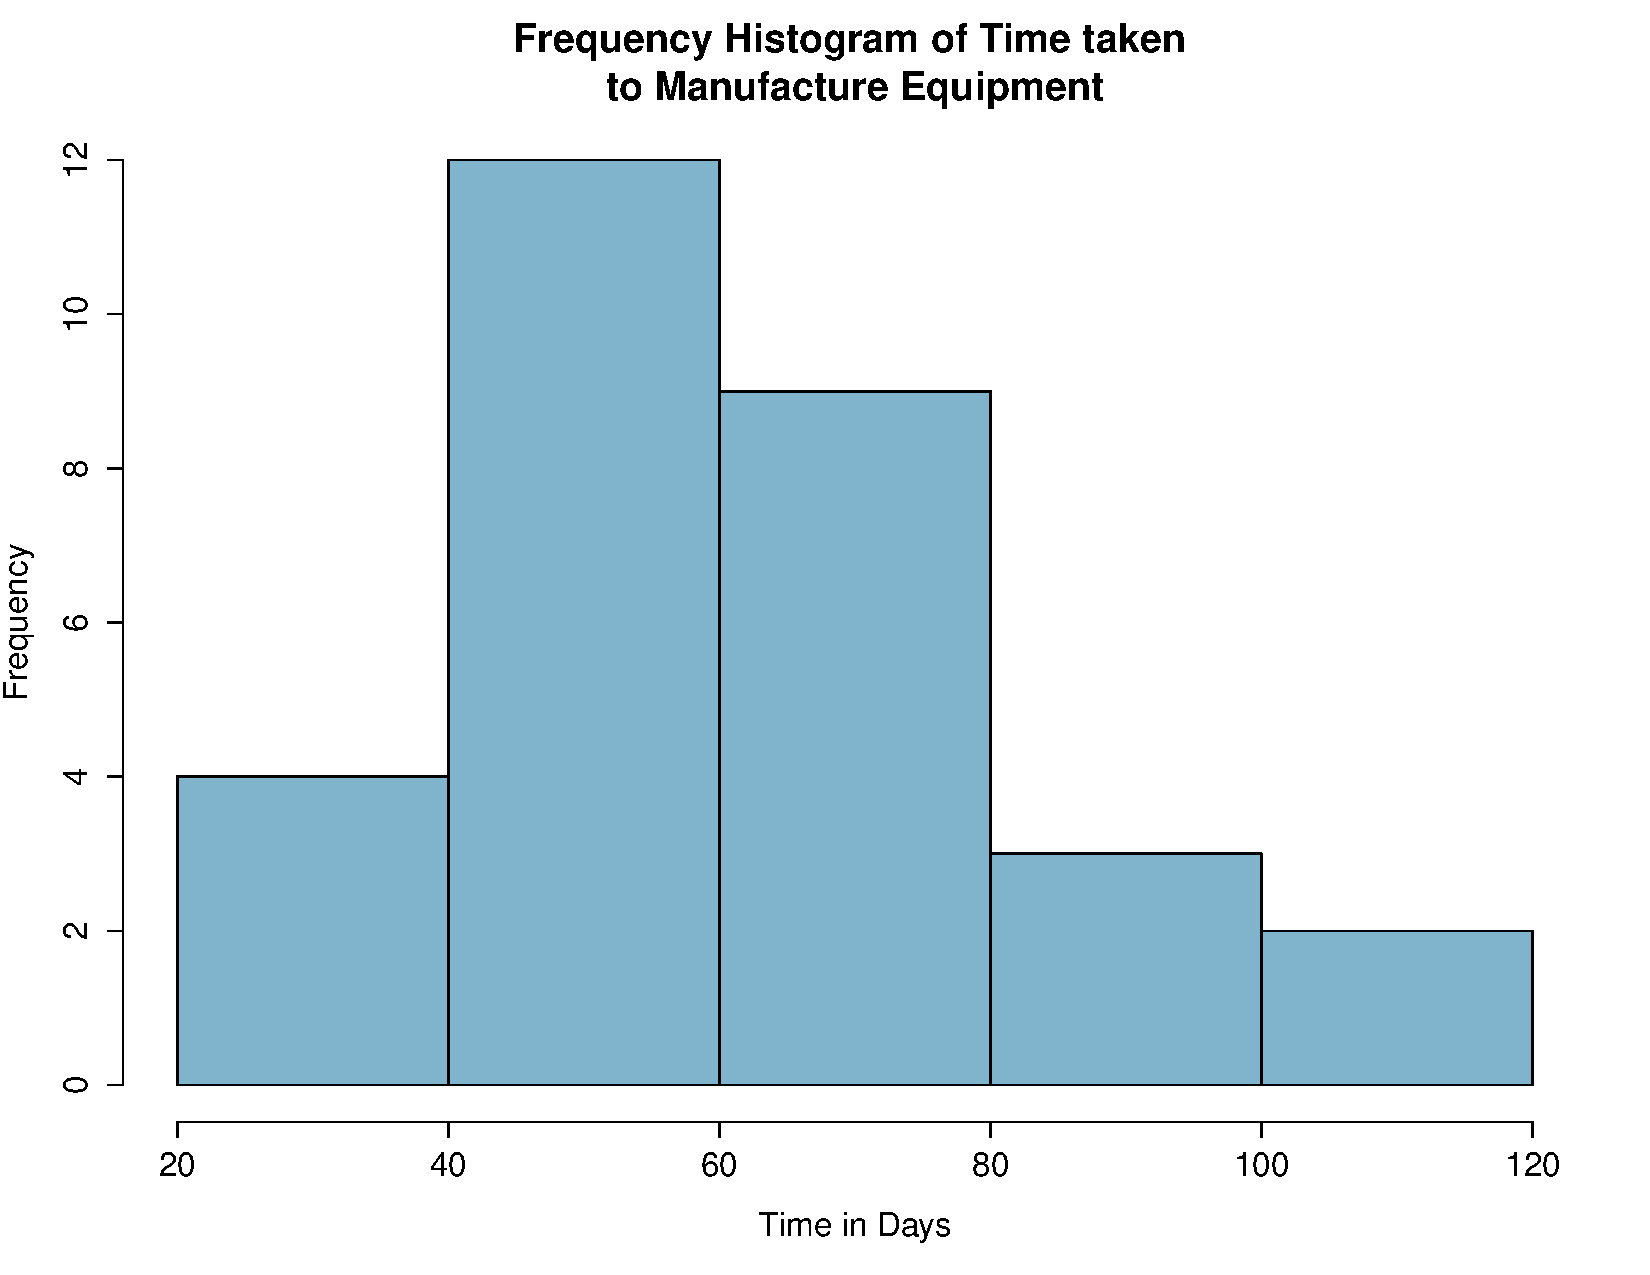
\includegraphics[scale=0.27]{Section2/freq_hist.pdf}	&	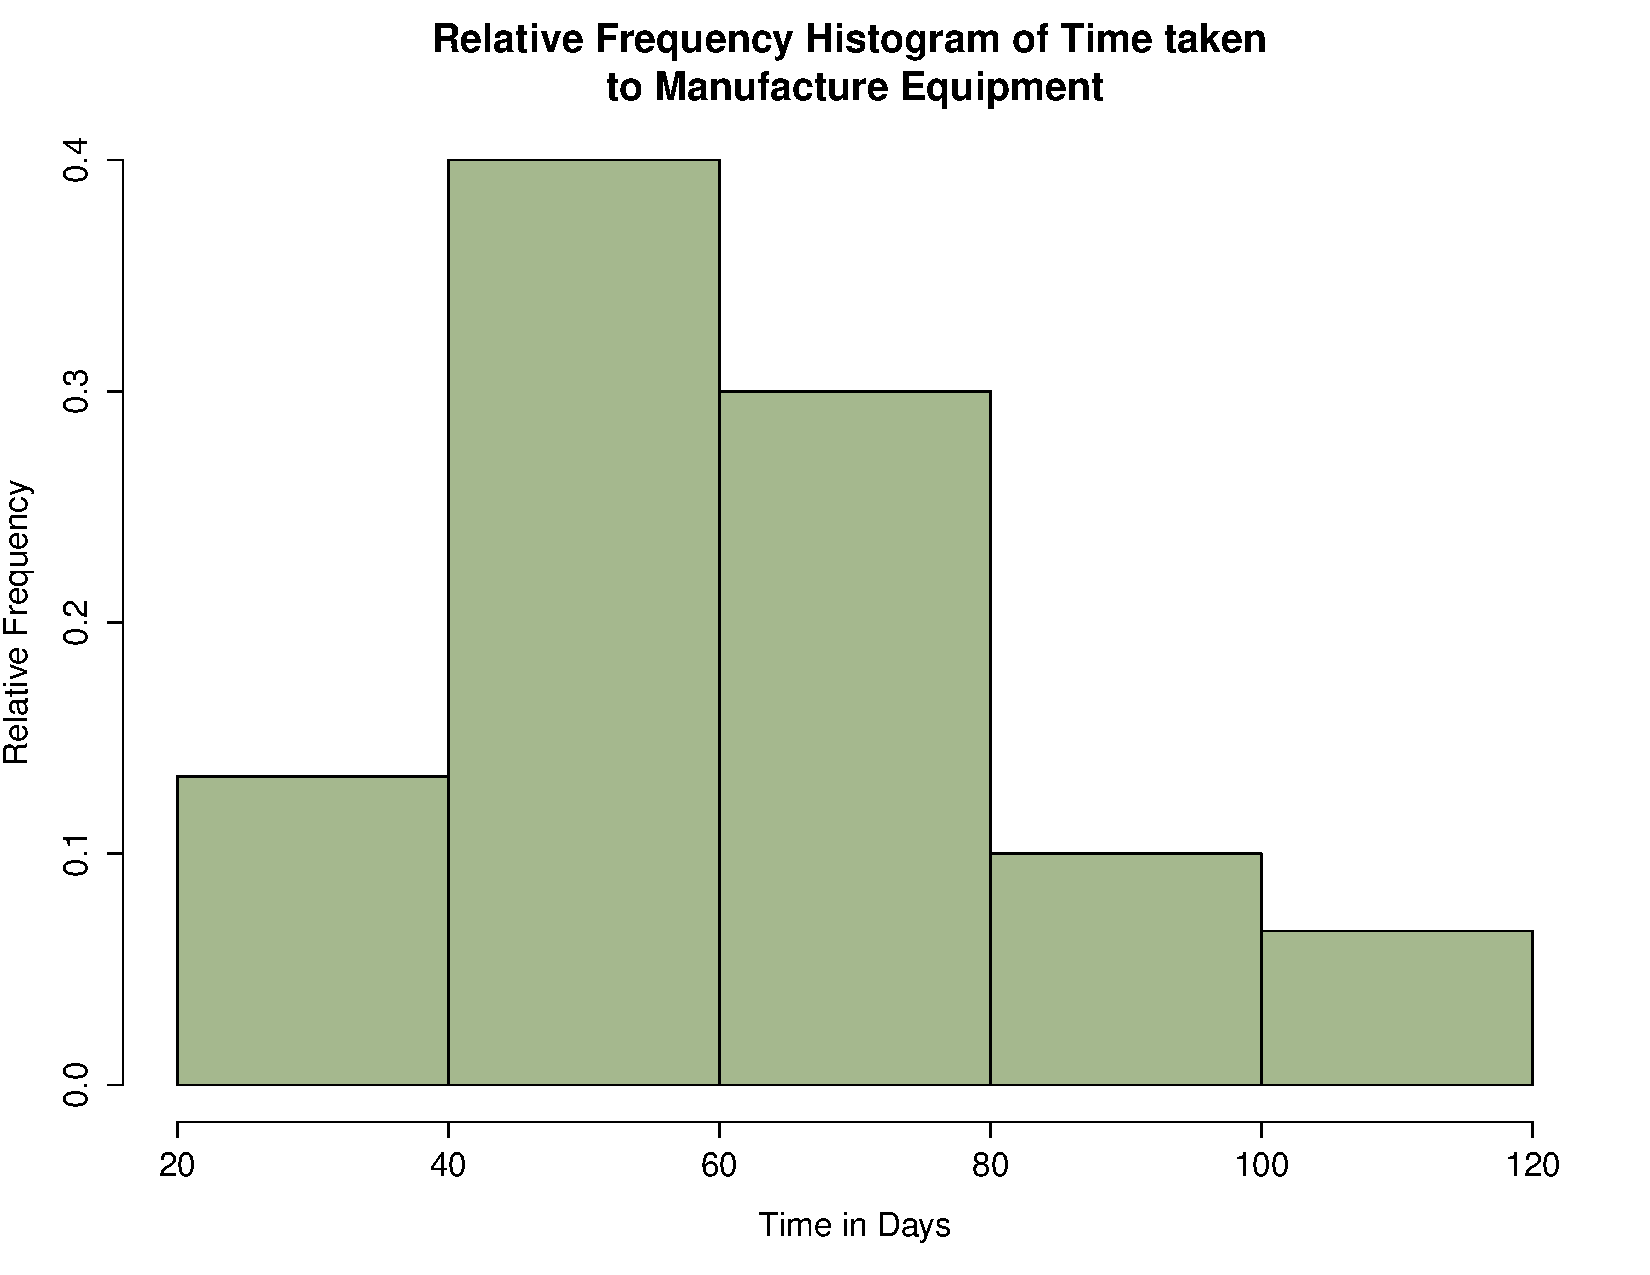
\includegraphics[scale=0.27]{Section2/rel_freq_hist.pdf}
\end{tabular}
\end{center}

Through visual inspection of the histograms, it appears as though the distribution of our data is right skewed. We can therefore deduce that the mean is less than the median.

\end{example}

\subsection{Boxplots}\label{sectionBoxplots}
\index{Boxplots}
\index{Plots!Bosplots}

\textit{Boxplots} are another visual aid we can use to present and interpret data.
They are one of the most simple graphical techniques to analyze visually.
Boxplots are also known as \textit{box-and-whisker plots} since they consists of
figures resembling boxes along with a series of lines which we refer to as whiskers.
The whiskers represent the quartiles as well as special values which we refer to as
the \textit{lower whisker} and the \textit{upper whisker}.

\begin{definition}[Upper \& Lower Whiskers]
Let $Q_{1}$, $Q_{3}$ and $IQR$ represent the first quartile, third quartile and 
interquartile range respectively. Then,
\[ \text{Lower Whisker} ~ = ~ Q_{1} - 1.5 \times IQR \]
\[ \text{Upper Whisker} ~ = ~ Q_{3} + 1.5 \times IQR \]
\end{definition}

\noindent
Boxplots are very useful tool for identifying outliers as they are any values which fall outside of the lower and upper whiskers. We can also use boxplots to obtain information regarding the skewness of data. We achieve this by analyzing how close the quartiles are to each other graphically.\\

\noindent
To construct a boxplot:
\begin{enumerate}
\item Draw whiskers at the values
of the lower whisker and the upper whisker.
\item Draw the box around the values of the quartiles. The top of the box represents $Q_3$, the bottom of the box represents $Q_1$, and the line within the box represents the median or $Q_2$.
\item Any values that are greater than the upper whisker or less than the lower whisker are outliers and are represented by single points.
\end{enumerate}

\begin{nt}
Boxplots can be oriented horizontally or vertically and the width of the boxplot does not have any significance.
\end{nt}

\begin{figure}[H]

\begin{center}
%\scalebox{0.9}{
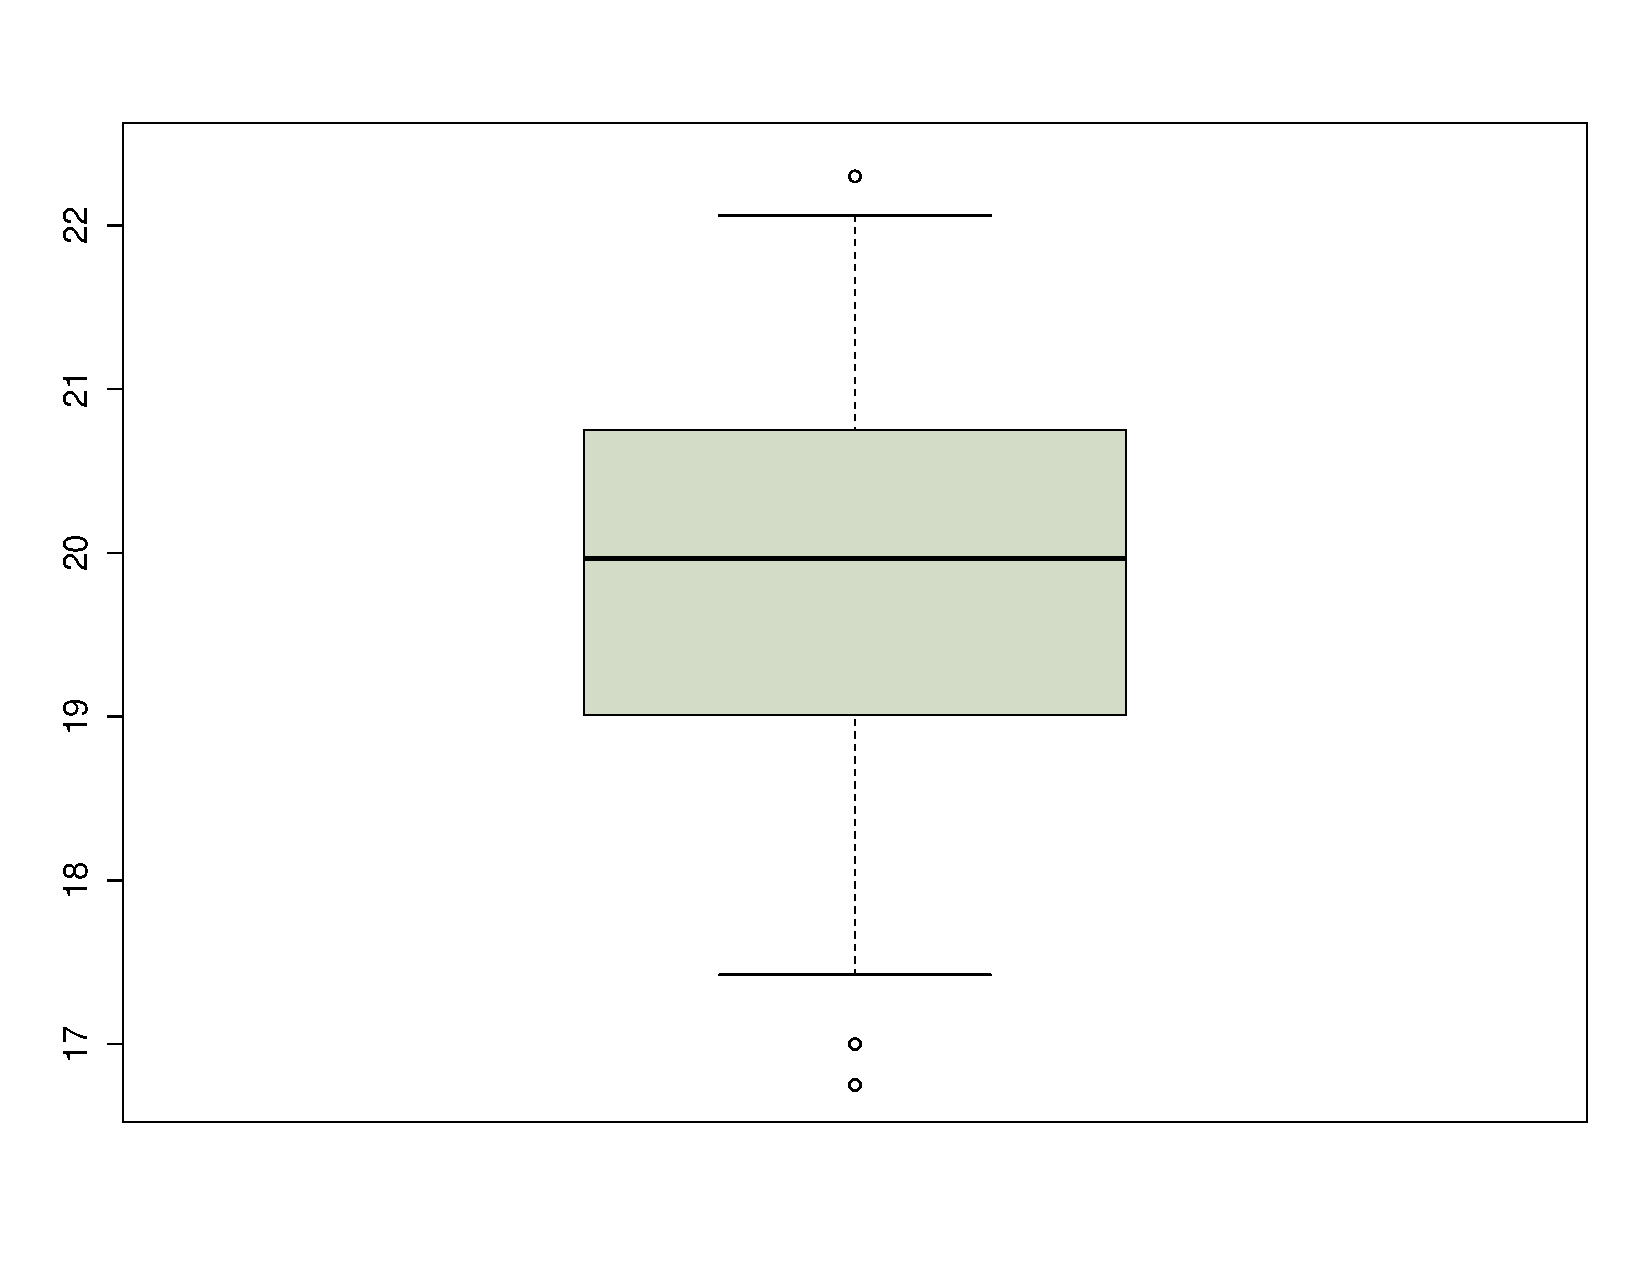
\includegraphics[scale=0.50]{Section2/boxplot.pdf}

%\begin{picture}(0,0)
%\put(0,0){ 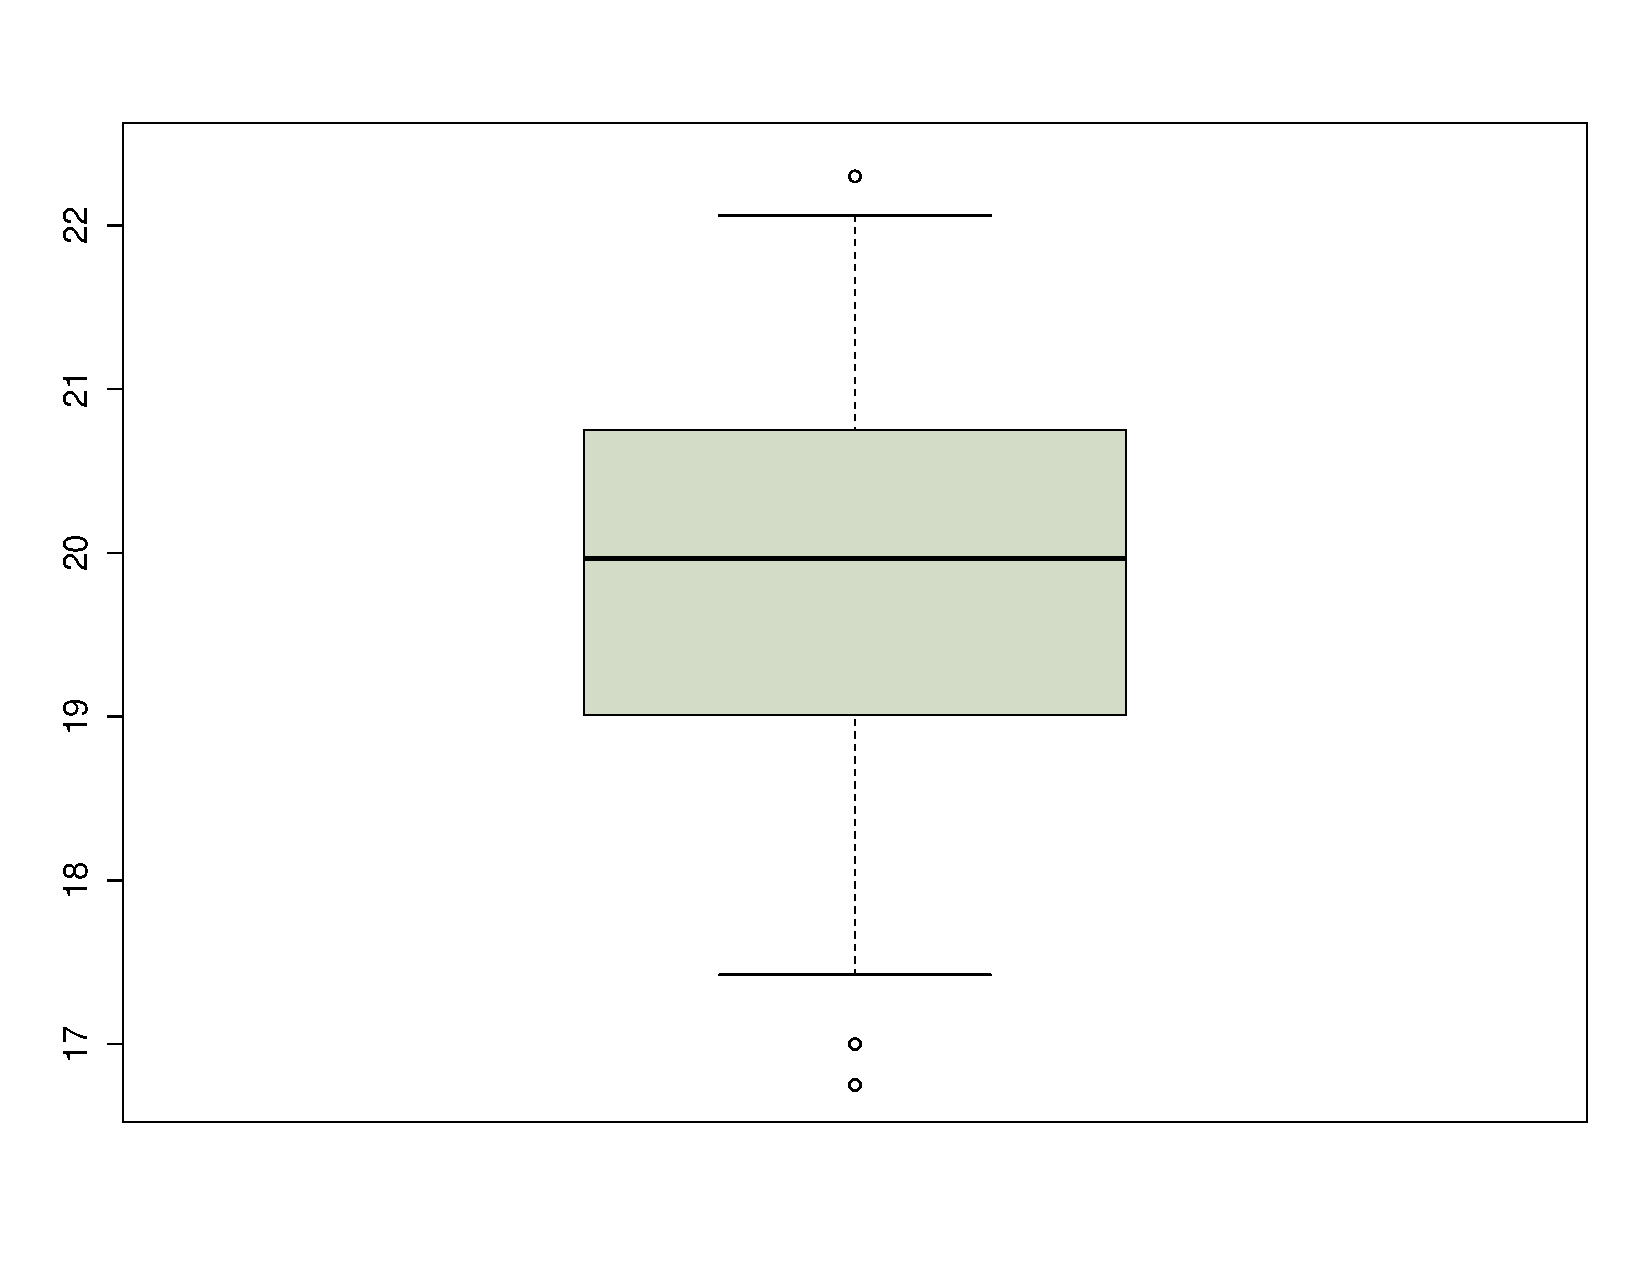
\includegraphics[scale=0.450]{Section2/boxplot.pdf} } 
%
%\put(-25,140){\hbox{ \scriptsize{Q$_{3}$} } }
%\put(-25,118){\hbox{ \scriptsize{Q$_{2}$} } }
%\put(-25,93){\hbox{ \scriptsize{Q$_{1}$} } }
%
%\put(176,48){\hbox{ \scriptsize{Q$_{1} $} --- 1.5(IQR) } }
%\put(176,178){\hbox{ \scriptsize{Q$_{3} $} + 1.5(IQR) } }
%
%\put(150, 32.5){ $\}$ }
%\put(155.0,33.0){ \hbox{ \scriptsize{outliers} } }
%
%\put(135.5,183.0){ $\{$ }
%\put(104,184){ \hbox{ \scriptsize{outliers} } }
%
%
%%\put(-10, 215.0){ \hbox{How to interpret a boxplot } }
%
%%\put(225,150){\hbox{mean	\quad\quad	median}}
%\end{picture}

\begin{tikzpicture}[overlay]
\draw [dashed] (2.0, 7.575) -- (5, 7.575);
\draw [dashed] (2.0, 6.49) -- (5, 6.49);
\draw [dashed] (2.0, 5.1625) -- (5, 5.1625);
%\put (2.0, 5.2){\hbox{\quad Q3}}

\node[text width=4cm] at (0.6, 9.7) {Outliers $\{$ };

\node[text width=4cm] at (4, 9.4) {Q$_{3}$ + 1.5(IQR)};
\node[text width=4cm] at (7.2, 7.6) {Q$_{3}$};
\node[text width=4cm] at (7.2, 6.4) {Q$_{2}$};
\node[text width=4cm] at (7.2, 5.1) {Q$_{1}$};
\node[text width=4cm] at (4, 3.0) {Q$_{1}$  $-$ 1.5(IQR)};

\node[text width=4cm] at (0.6, 2.2) {Outliers $\{$ };

\end{tikzpicture}
%}
\end{center}

\vspace*{-1.75cm}
\caption{Interpreting a boxplot}
\end{figure}


We can also perform a side by side comparison of several boxplots 
in order to compare the skewness of different data sets,
such as in figure $\ref{figureSideBySideBoxplotComparison}$.


\begin{figure}[H]
\label{figureSideBySideBoxplotComparison}
\begin{center}
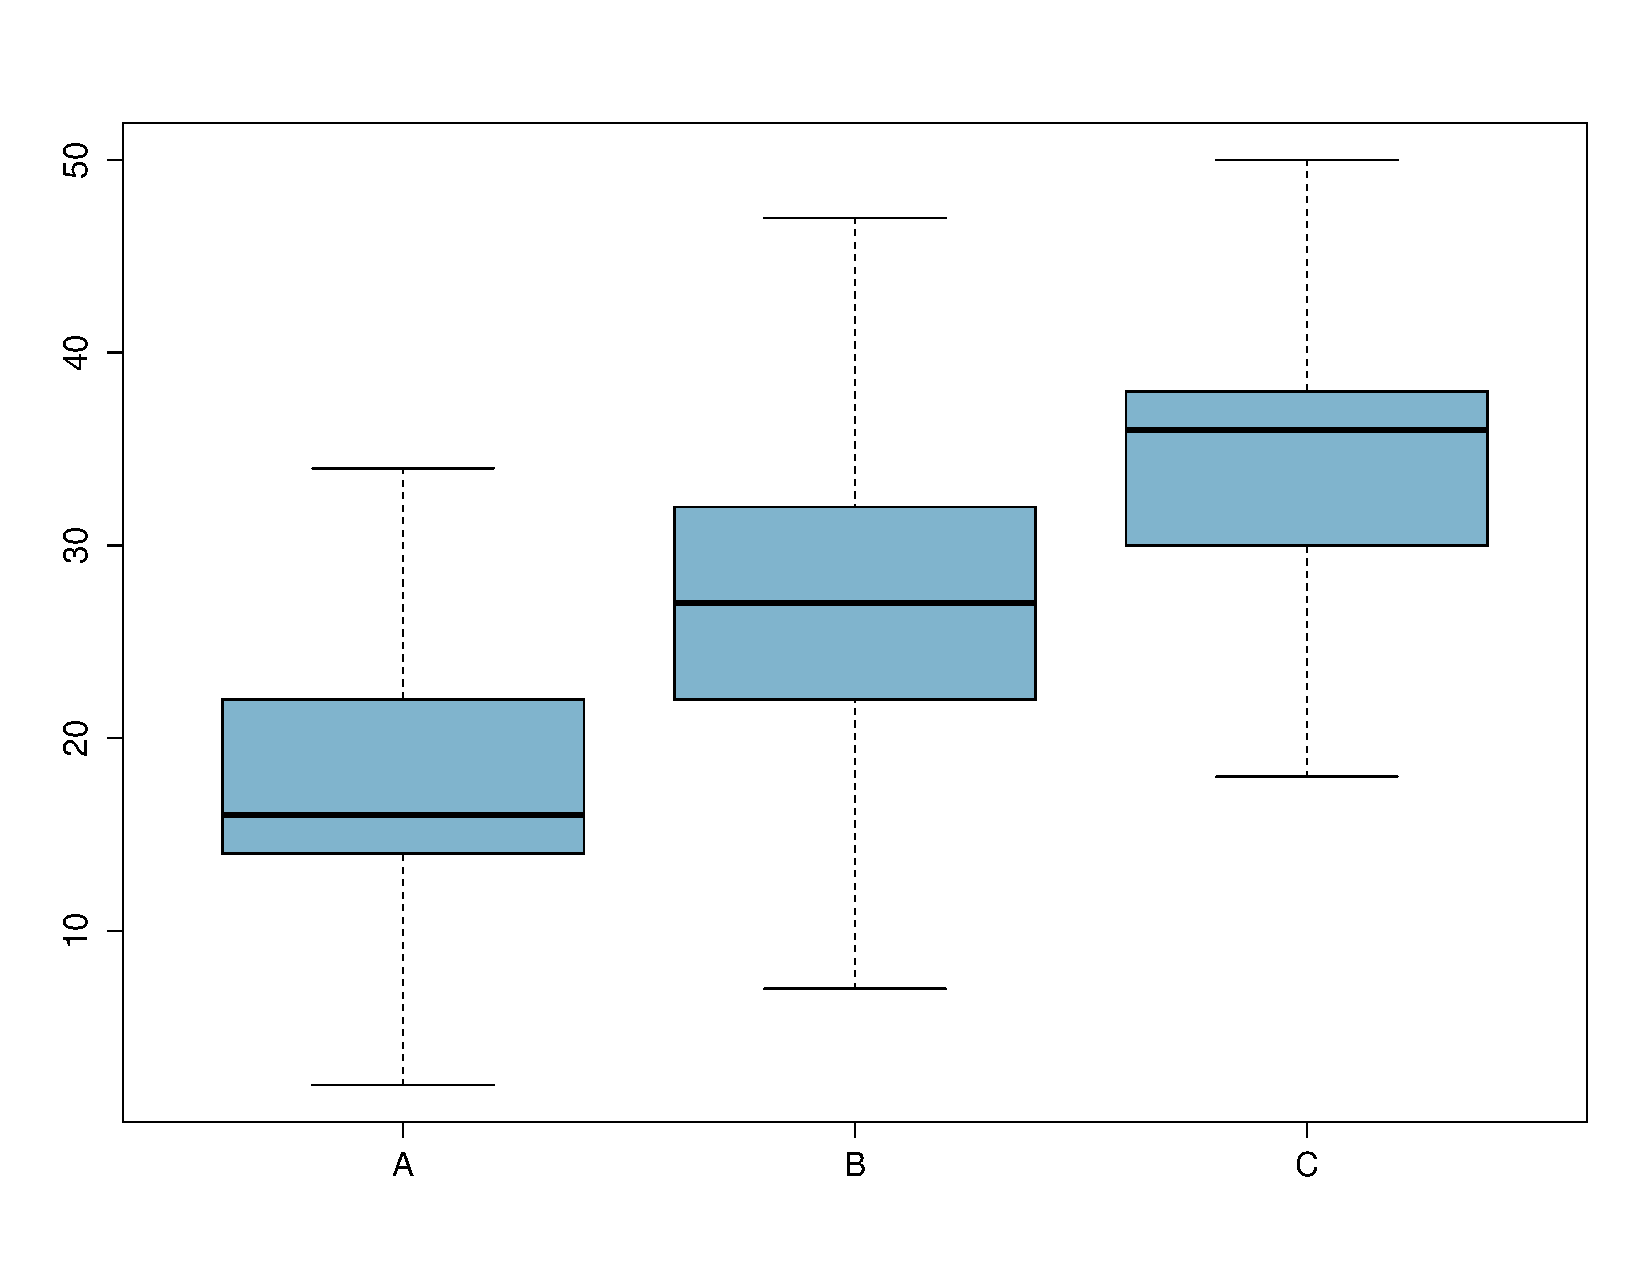
\includegraphics[scale=0.4]{Section2/boxplot_abc.pdf}
\end{center}
\vspace*{-0.75cm}
\caption{A positively skewed boxplot (A), a symmetric boxplot (B) and a negatively skewed boxplot (C)}
\end{figure}
%\end{center}

\begin{example}
Suppose we have the following $n=10$ observations:
\begin{center}
\begin{tabular}{cccccccccc}
26 & 20 & 26 & 19 & 25 & 16 & 10 & 33 & 43 & 17
\end{tabular} 
\end{center}

\noindent
Construct a boxplot for this data.

\hfill\\
{\emph{\textbf{\underline{Solution:}}}}\\

\noindent
First, we find the median. Since $n=10$ is even, the median is the average of the fifth and sixth ordered observations. 

\[Median = \frac{20+25}{2} = 22.5\]

\noindent
Splitting the data into two sets yields

\begin{center}
\def\arraystretch{1.5}
\begin{tabular}{ccccc}
10 & 16 & \underline{17} & 19 & 20 \\  
25 & 26 & \underline{26} & 33 & 43 \\ 
\end{tabular} 
\end{center}

Therefore, $Q_1=17$ and $Q_3=26$. We can now calculate the IQR and the whiskers.
\[ IQR = Q_3-Q_1 =27-17=10\]
\[ \text{Lower whisker} = Q_1-1.5 \times IQR = 17 - 1.5(10) =  2 \]
\[ \text{Upper whisker} = Q_3+1.5 \times IQR = 26 + 1.5(10) = 41 \]

The observation of 43 falls outside of the upper whisker and is therefore an outlier. 

\begin{center}
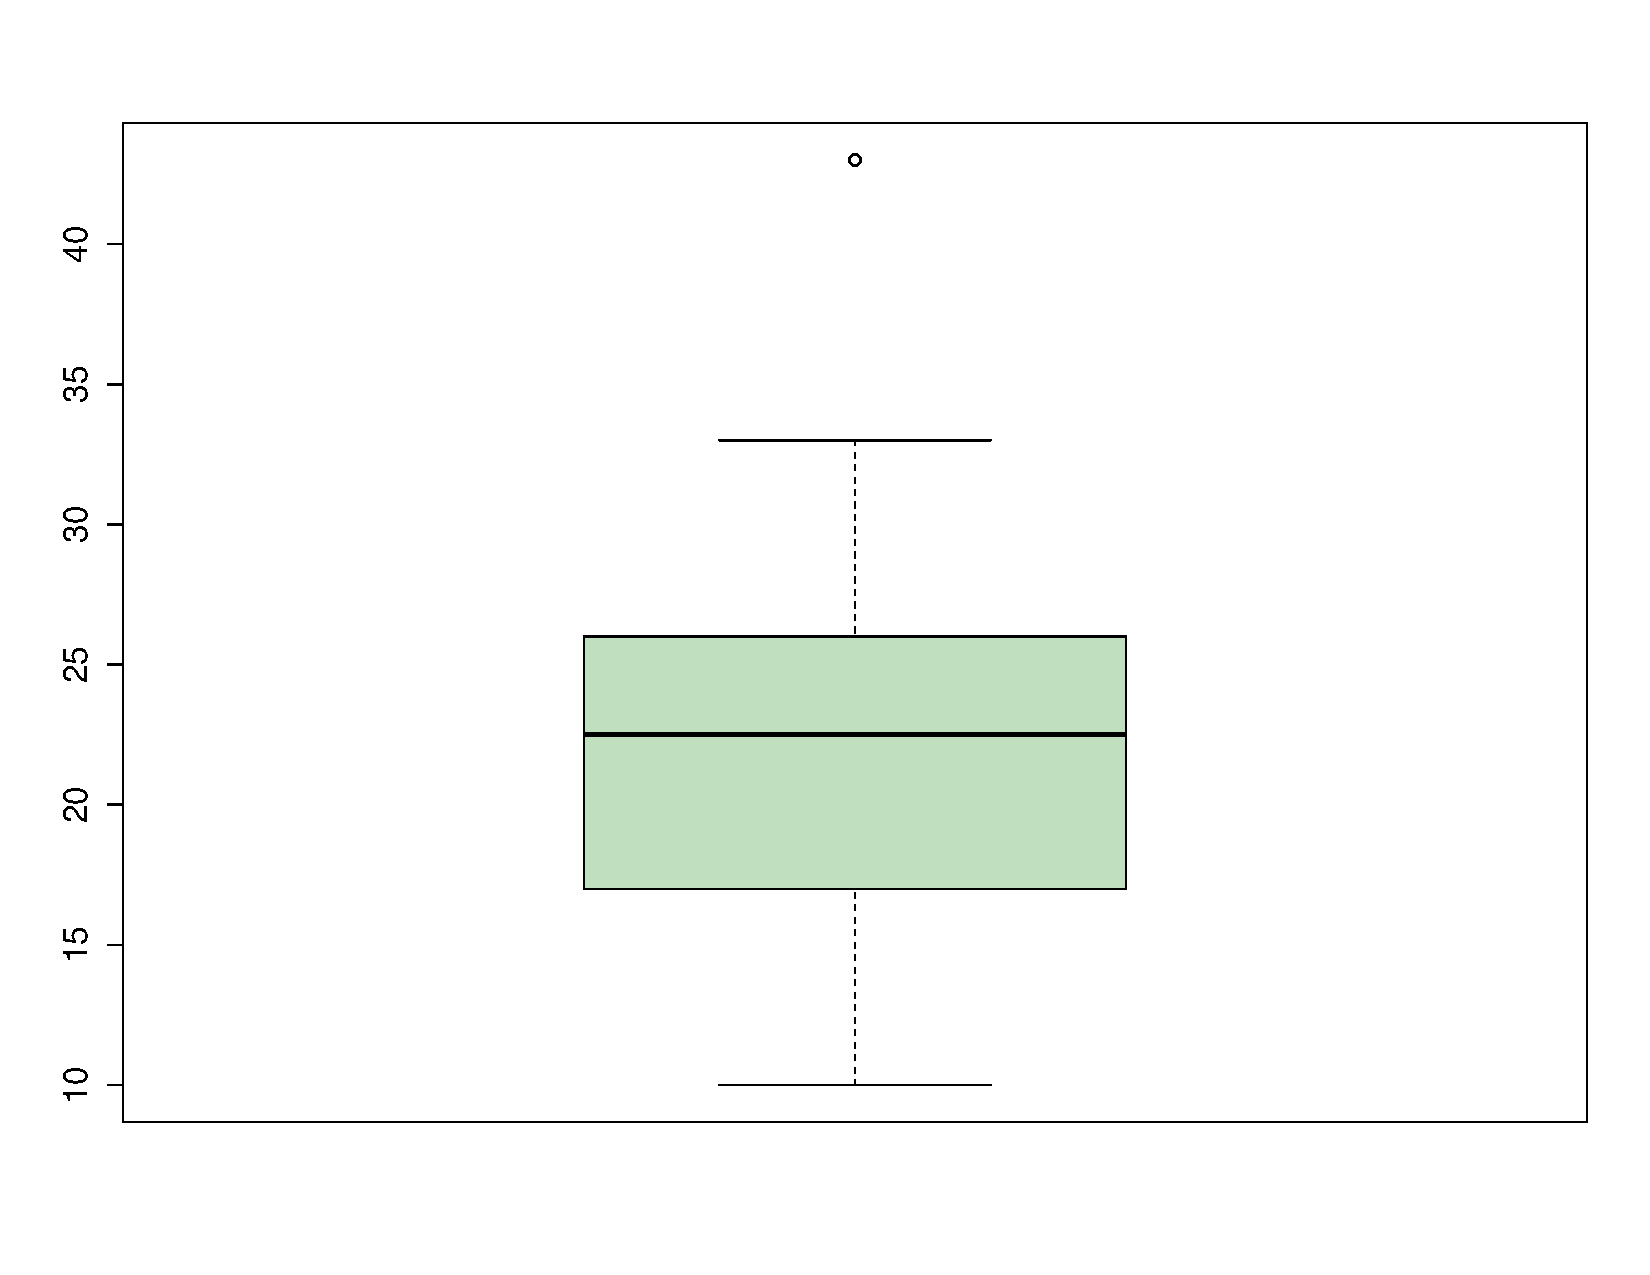
\includegraphics[scale=0.25]{Section2/boxplotex.pdf}
\end{center}

\noindent
The upper whisker is drawn at the highest value below 41 which is 33. The lower whisker is drawn at the lowest value above 2 which is 10. The outlier of 43 is represented by a circle. The boxplot appears to suggest that the distribution may be slightly negatively (or left) skewed.

\end{example}

\pagebreak


\subsection{Stem and Leaf Plots}
\index{Plots!Stem and leaf plots}
\index{Stem and leaf plots}

A \textit{stem and leaf plot} (sometimes referred to as simply a \textit{stem plot}) is a tabular method of displaying data.
Each observation is split into a \textit{stem} (the ``larger'' part of an observation) and a \textit{leaf} (the smaller part of an observation).\\

\vspace*{-0.50em}

One common partition is to let the stem represent a whole number and the leaves represent the decimal part of the number.
Another common partition is to consider the stem to be the integer part of some power of 10 (ex. 10, 100, 1000 etc.) Stem and leaf plots are easier to understand with the aid of an example.

\begin{example}
Consider the following set of (sorted) data points:
\begin{center}
\begin{tabular}{c c c c c c c c c c}
10.1	&	10.1	&	10.2	&	10.3	&	11.1	&	11.2	&	11.2	&	11.2	&	11.3	&	12.0	\\ 
12.0	&	12.3	&	12.4	&	12.5	&	12.5	&	12.6	&	14.2	&	14.2	&	14.3	&	14.3	\\
14.4	&	15.1	&	15.2	&	15.3	&	15.3	&	16.0	&	16.1	&	16.2	&	 18.0	&	18.1
\end{tabular}
\end{center}

Create a stem and leaf plot for this data.

\vspace*{-0.50em}

\hfill\\
{\emph{\textbf{\underline{Solution:}}}}\\

\noindent
Let's group terms and rewrite our data as follows:
\begin{center}
\begin{tabular}{c c c c c c c c c c}
10.1	&	10.1	&	10.2	&	10.3	\\ 
11.1	&	11.2	&	11.2	&	11.2	&	11.3	\\
12.0	&	12.0	&	12.3	&	12.4	&	12.5	&	12.5	&	12.6	\\
14.2	&	14.2	&	14.3	&	14.3	&	14.4	\\	
15.1	&	15.2	&	15.3	&	15.3	\\
16.0	&	16.1	&	16.2	\\
18.0	&	18.1	\\
\end{tabular}
\end{center}

\noindent
We can now construct out stem and leaf plot. 
Let's choose our partition ($|$) to be at the decimal point.
As such, the stem and leaf plot for this data is:\\

\vspace*{-0.50em}

\begin{center}
\begin{tabular}{r c l}
%\hfill\\
10	&	$|$	&	1123		\\
11	&	$|$	&	12223	\\
12	&	$|$	&	0034556	\\
13	&	$|$	&			\\
14	&	$|$	&	22334	\\
15	&	$|$	&	1233		\\
16	&	$|$	&	012		\\
17	&	$|$	&			\\
18	&	$|$	&	01
\end{tabular}
\end{center}
\end{example}